\section{Experiments}
\label{sec:results}

\subsection{Setup}

\paragraph{Benchmarks.} JAHS-Bench-201~\citep{bansal2022jahsbench} on all three of its built-in datasets
(CIFAR-10, Colorectal-Histology, Fashion-MNIST), and NAS-HPO-Bench-II~\citep{hirose2021nashpobenchii} within its
exhaustively tabulated 12-epoch range. The three JAHS-Bench-201 datasets test robustness within one benchmark
family, not generalisation beyond it.

\paragraph{Arms.} Table~\ref{tab:ablation-grid} organises the engine and surrogate ablations. NSGANetV2 is the
primary baseline; NSGA-Net and P3-alone are the surrogate-free versions of each engine; P3+abs.\ regressor
isolates the surrogate on P3Net's own engine. P3-alone originally used a population of 10 against 20 for every
other population-based arm, so two further arms, P3-alone-pop20 and P3-alone-pop40, remove that confound. Outside
the grid we compare against SH-EMOA~\citep{beume2007smsemoa} and MO-BOHB~\citep{falkner2018bohb}, established for
this joint setting~\citep{guerreroviu2021bagofbaselines}, and against TPE~\citep{bergstra2011tpe} and uniform
random search. The relative surrogate is defined only given a linkage tree, so an NSGA-II-plus-relative cell
cannot be built; the grid separates engine and surrogate as far as that permits. The surrogate ablation is
also not purely a change of formulation: P3Net's $\hat\delta_F$ uses ridge regression, while P3+abs.\ regressor
and NSGANetV2 use unregularised linear regression.

\begin{table}[t]
    \centering
    \caption{Engine/surrogate ablation grid. The NSGA-II/relative cell is not constructible. SH-EMOA, MO-BOHB,
    TPE, random search, and the two P3-alone population variants complete the eleven arms.}
    \label{tab:ablation-grid}
    \begin{tabular}{@{}lccc@{}}
        \toprule
         & \textbf{None} & \textbf{Absolute} & \textbf{Relative} $\hat{\delta}_F$ \\
        \midrule
        \textbf{NSGA-II} & NSGA-Net & NSGANetV2 & --- \\
        \textbf{P3}      & P3-alone & P3+abs.\ regressor & P3Net \\
        \bottomrule
    \end{tabular}
\end{table}

\paragraph{Fairness controls.} All arms share the genotype encoding, discretised hyperparameter grid, decoder,
validity check, full-evaluation budget, seed list, and deduplication cache. Discretising $\Theta$ equalises
resolution but is not neutral: it removes the real-valued crossover a native NSGANetV2 extension would use while
costing P3 nothing. A control arm running NSGANetV2 on continuous $\Theta$ was not completed, so this asymmetry is
acknowledged but not bounded. Budgets count full evaluations only; the surrogate arms additionally spend
wall-clock time on refitting and, for the P3 engine, on rebuilding the linkage tree, which we do not equalise.

\paragraph{Budgets and seeds.} Four tiers of $\{50, 100, 200, 350\}$ full evaluations. The second matches
JAHS-Bench-201's suggested protocol of about 100 evaluations~\citep{bansal2022jahsbench}; the largest matches the
full-evaluation count NSGANetV2 reports~\citep{lu2020nsganetv2}. All tiers are below NAS-HPO-Bench-II's
500-trial convention, deliberately, since the question concerns a limited budget. $R=30$ independent runs per
arm, per cell, with a fixed published seed list.

\paragraph{Metrics.} On NAS-HPO-Bench-II we enumerate all 196608 configurations, of which 188496 are valid,
and obtain the exact oracle Pareto front (25 points). We report IGD+ against it, with both objectives normalised
to the oracle front's range; across that front the training-time objective spans 18.53 times the range of the
error objective, so without normalisation it would dominate the distance. JAHS-Bench-201 admits no enumerable front, so we report hypervolume relative to a
best-known front: the nondominated set of every point evaluated by any arm, any budget, and any seed, pooled per
dataset. That front is computed once, persisted, and reused for every table, so adding an arm cannot retroactively
change the denominator of existing results.

\paragraph{Statistics.} P3Net is compared against each of the other ten arms, per (search space, budget) cell,
with paired Wilcoxon signed-rank tests, Holm--Bonferroni correction within the cell, and Cliff's $\delta$
reported for every comparison, following benchmarking practice for stochastic
optimisers~\citep{BartzBeielstein2020Benchmarking,Hansen2016b}. We orient $\delta$ so that a positive value
favours P3Net on both metrics.

\subsection{Headline comparison}

Tables~\ref{tab:heatmap-jahs}--\ref{tab:heatmap-nashpo} give Cliff's $\delta$ of P3Net against every other arm in
every cell; the supplementary material lists medians, IQRs, and corrected $p$-values.

% GENERATED by implementation/experiments/scripts/render_results_tex.py.
% Do not edit by hand -- regenerate from results/tables/ instead.

\begin{table}[t]
    \centering
    \footnotesize
    \caption{Effect-size heatmap, CIFAR-10: Cliff's $\delta$ of P3Net vs.\ each baseline on hypervolume relative to the frozen best-known front (higher is better). Blue favours P3Net, red favours the baseline; darker is larger $|\delta|$. Boxed cells reject $H_0$ at $\alpha=0.05$ (Holm--Bonferroni, per cell).}
    \label{tab:heatmap-jahs}
    \begin{tabular}{@{}lcccc@{}}
        \toprule
        \textbf{Method} & \textbf{50} & \textbf{100} & \textbf{200} & \textbf{350} \\
        \midrule
        P3-alone & \fcolorbox[HTML]{000000}{3987E5}{\makebox[2.4em]{\textcolor{white}{\textbf{+0.53}}}} & \fcolorbox[HTML]{000000}{184F95}{\makebox[2.4em]{\textcolor{white}{\textbf{+0.77}}}} & \fcolorbox[HTML]{000000}{184F95}{\makebox[2.4em]{\textcolor{white}{\textbf{+0.80}}}} & \fcolorbox[HTML]{000000}{86B6EF}{\makebox[2.4em]{\textcolor{black}{\textbf{+0.49}}}} \\
        P3-alone-pop20 & \colorbox[HTML]{86B6EF}{\makebox[2.4em]{\textcolor{black}{+0.36}}} & \fcolorbox[HTML]{000000}{3987E5}{\makebox[2.4em]{\textcolor{white}{\textbf{+0.55}}}} & \fcolorbox[HTML]{000000}{3987E5}{\makebox[2.4em]{\textcolor{white}{\textbf{+0.59}}}} & \fcolorbox[HTML]{000000}{3987E5}{\makebox[2.4em]{\textcolor{white}{\textbf{+0.58}}}} \\
        P3-alone-pop40 & \colorbox[HTML]{EAF2FC}{\makebox[2.4em]{\textcolor{black}{+0.05}}} & \fcolorbox[HTML]{000000}{86B6EF}{\makebox[2.4em]{\textcolor{black}{\textbf{+0.46}}}} & \fcolorbox[HTML]{000000}{86B6EF}{\makebox[2.4em]{\textcolor{black}{\textbf{+0.36}}}} & \colorbox[HTML]{CDE2FB}{\makebox[2.4em]{\textcolor{black}{+0.21}}} \\
        P3+abs.\ regressor & \colorbox[HTML]{EAF2FC}{\makebox[2.4em]{\textcolor{black}{+0.09}}} & \colorbox[HTML]{CDE2FB}{\makebox[2.4em]{\textcolor{black}{+0.14}}} & \colorbox[HTML]{CDE2FB}{\makebox[2.4em]{\textcolor{black}{+0.16}}} & \colorbox[HTML]{CDE2FB}{\makebox[2.4em]{\textcolor{black}{+0.17}}} \\
        \midrule
        NSGA-Net & \colorbox[HTML]{86B6EF}{\makebox[2.4em]{\textcolor{black}{+0.31}}} & \colorbox[HTML]{CDE2FB}{\makebox[2.4em]{\textcolor{black}{+0.29}}} & \colorbox[HTML]{F2A3A2}{\makebox[2.4em]{\textcolor{black}{-0.38}}} & \fcolorbox[HTML]{000000}{941F1F}{\makebox[2.4em]{\textcolor{white}{\textbf{-0.89}}}} \\
        NSGANetV2 & \colorbox[HTML]{EAF2FC}{\makebox[2.4em]{\textcolor{black}{+0.07}}} & \colorbox[HTML]{FDEEED}{\makebox[2.4em]{\textcolor{black}{-0.02}}} & \colorbox[HTML]{FBDCDB}{\makebox[2.4em]{\textcolor{black}{-0.26}}} & \colorbox[HTML]{F2A3A2}{\makebox[2.4em]{\textcolor{black}{-0.39}}} \\
        \midrule
        MO-BOHB & \colorbox[HTML]{FBDCDB}{\makebox[2.4em]{\textcolor{black}{-0.12}}} & \colorbox[HTML]{86B6EF}{\makebox[2.4em]{\textcolor{black}{+0.35}}} & \fcolorbox[HTML]{000000}{86B6EF}{\makebox[2.4em]{\textcolor{black}{\textbf{+0.46}}}} & \colorbox[HTML]{CDE2FB}{\makebox[2.4em]{\textcolor{black}{+0.28}}} \\
        random search & \colorbox[HTML]{EAF2FC}{\makebox[2.4em]{\textcolor{black}{+0.05}}} & \colorbox[HTML]{CDE2FB}{\makebox[2.4em]{\textcolor{black}{+0.12}}} & \colorbox[HTML]{CDE2FB}{\makebox[2.4em]{\textcolor{black}{+0.17}}} & \colorbox[HTML]{CDE2FB}{\makebox[2.4em]{\textcolor{black}{+0.25}}} \\
        SH-EMOA & \colorbox[HTML]{FBDCDB}{\makebox[2.4em]{\textcolor{black}{-0.17}}} & \fcolorbox[HTML]{000000}{F2A3A2}{\makebox[2.4em]{\textcolor{black}{\textbf{-0.49}}}} & \fcolorbox[HTML]{000000}{941F1F}{\makebox[2.4em]{\textcolor{white}{\textbf{-0.88}}}} & \fcolorbox[HTML]{000000}{941F1F}{\makebox[2.4em]{\textcolor{white}{\textbf{-0.96}}}} \\
        TPE & \colorbox[HTML]{FBDCDB}{\makebox[2.4em]{\textcolor{black}{-0.30}}} & \colorbox[HTML]{FBDCDB}{\makebox[2.4em]{\textcolor{black}{-0.28}}} & \fcolorbox[HTML]{000000}{E34948}{\makebox[2.4em]{\textcolor{white}{\textbf{-0.70}}}} & \fcolorbox[HTML]{000000}{941F1F}{\makebox[2.4em]{\textcolor{white}{\textbf{-0.82}}}} \\
        \bottomrule
    \end{tabular}
\end{table}

\begin{table}[t]
    \centering
    \footnotesize
    \caption{Effect-size heatmap, Colorectal-Histology: Cliff's $\delta$ of P3Net vs.\ each baseline on hypervolume relative to the frozen best-known front (higher is better). Blue favours P3Net, red favours the baseline; darker is larger $|\delta|$. Boxed cells reject $H_0$ at $\alpha=0.05$ (Holm--Bonferroni, per cell).}
    \label{tab:heatmap-colorectal}
    \begin{tabular}{@{}lcccc@{}}
        \toprule
        \textbf{Method} & \textbf{50} & \textbf{100} & \textbf{200} & \textbf{350} \\
        \midrule
        P3-alone & \fcolorbox[HTML]{000000}{3987E5}{\makebox[2.4em]{\textcolor{white}{\textbf{+0.67}}}} & \fcolorbox[HTML]{000000}{3987E5}{\makebox[2.4em]{\textcolor{white}{\textbf{+0.61}}}} & \fcolorbox[HTML]{000000}{86B6EF}{\makebox[2.4em]{\textcolor{black}{\textbf{+0.44}}}} & \colorbox[HTML]{FDEEED}{\makebox[2.4em]{\textcolor{black}{-0.04}}} \\
        P3-alone-pop20 & \fcolorbox[HTML]{000000}{86B6EF}{\makebox[2.4em]{\textcolor{black}{\textbf{+0.44}}}} & \colorbox[HTML]{86B6EF}{\makebox[2.4em]{\textcolor{black}{+0.32}}} & \colorbox[HTML]{FBDCDB}{\makebox[2.4em]{\textcolor{black}{-0.14}}} & \colorbox[HTML]{FBDCDB}{\makebox[2.4em]{\textcolor{black}{-0.18}}} \\
        P3-alone-pop40 & \colorbox[HTML]{EAF2FC}{\makebox[2.4em]{\textcolor{black}{+0.06}}} & \colorbox[HTML]{FDEEED}{\makebox[2.4em]{\textcolor{black}{+0.00}}} & \colorbox[HTML]{FBDCDB}{\makebox[2.4em]{\textcolor{black}{-0.30}}} & \fcolorbox[HTML]{000000}{E34948}{\makebox[2.4em]{\textcolor{white}{\textbf{-0.54}}}} \\
        P3+abs.\ regressor & \colorbox[HTML]{CDE2FB}{\makebox[2.4em]{\textcolor{black}{+0.27}}} & \colorbox[HTML]{EAF2FC}{\makebox[2.4em]{\textcolor{black}{+0.08}}} & \colorbox[HTML]{FBDCDB}{\makebox[2.4em]{\textcolor{black}{-0.12}}} & \colorbox[HTML]{FBDCDB}{\makebox[2.4em]{\textcolor{black}{-0.19}}} \\
        \midrule
        NSGA-Net & \colorbox[HTML]{CDE2FB}{\makebox[2.4em]{\textcolor{black}{+0.15}}} & \colorbox[HTML]{FDEEED}{\makebox[2.4em]{\textcolor{black}{-0.07}}} & \fcolorbox[HTML]{000000}{F2A3A2}{\makebox[2.4em]{\textcolor{black}{\textbf{-0.39}}}} & \fcolorbox[HTML]{000000}{941F1F}{\makebox[2.4em]{\textcolor{white}{\textbf{-0.82}}}} \\
        NSGANetV2 & \colorbox[HTML]{EAF2FC}{\makebox[2.4em]{\textcolor{black}{+0.08}}} & \fcolorbox[HTML]{000000}{F2A3A2}{\makebox[2.4em]{\textcolor{black}{\textbf{-0.48}}}} & \fcolorbox[HTML]{000000}{941F1F}{\makebox[2.4em]{\textcolor{white}{\textbf{-0.83}}}} & \fcolorbox[HTML]{000000}{941F1F}{\makebox[2.4em]{\textcolor{white}{\textbf{-0.81}}}} \\
        \midrule
        MO-BOHB & \colorbox[HTML]{CDE2FB}{\makebox[2.4em]{\textcolor{black}{+0.28}}} & \colorbox[HTML]{86B6EF}{\makebox[2.4em]{\textcolor{black}{+0.33}}} & \fcolorbox[HTML]{000000}{86B6EF}{\makebox[2.4em]{\textcolor{black}{\textbf{+0.49}}}} & \fcolorbox[HTML]{000000}{3987E5}{\makebox[2.4em]{\textcolor{white}{\textbf{+0.51}}}} \\
        random search & \colorbox[HTML]{EAF2FC}{\makebox[2.4em]{\textcolor{black}{+0.03}}} & \colorbox[HTML]{CDE2FB}{\makebox[2.4em]{\textcolor{black}{+0.20}}} & \colorbox[HTML]{CDE2FB}{\makebox[2.4em]{\textcolor{black}{+0.15}}} & \colorbox[HTML]{EAF2FC}{\makebox[2.4em]{\textcolor{black}{+0.08}}} \\
        SH-EMOA & \colorbox[HTML]{FDEEED}{\makebox[2.4em]{\textcolor{black}{-0.09}}} & \colorbox[HTML]{FBDCDB}{\makebox[2.4em]{\textcolor{black}{-0.28}}} & \fcolorbox[HTML]{000000}{941F1F}{\makebox[2.4em]{\textcolor{white}{\textbf{-0.80}}}} & \fcolorbox[HTML]{000000}{941F1F}{\makebox[2.4em]{\textcolor{white}{\textbf{-0.78}}}} \\
        TPE & \colorbox[HTML]{FBDCDB}{\makebox[2.4em]{\textcolor{black}{-0.20}}} & \colorbox[HTML]{FBDCDB}{\makebox[2.4em]{\textcolor{black}{-0.23}}} & \fcolorbox[HTML]{000000}{F2A3A2}{\makebox[2.4em]{\textcolor{black}{\textbf{-0.44}}}} & \fcolorbox[HTML]{000000}{F2A3A2}{\makebox[2.4em]{\textcolor{black}{\textbf{-0.45}}}} \\
        \bottomrule
    \end{tabular}
\end{table}

\begin{table}[t]
    \centering
    \footnotesize
    \caption{Effect-size heatmap, Fashion-MNIST: Cliff's $\delta$ of P3Net vs.\ each baseline on hypervolume relative to the frozen best-known front (higher is better). Blue favours P3Net, red favours the baseline; darker is larger $|\delta|$. Boxed cells reject $H_0$ at $\alpha=0.05$ (Holm--Bonferroni, per cell).}
    \label{tab:heatmap-fashion}
    \begin{tabular}{@{}lcccc@{}}
        \toprule
        \textbf{Method} & \textbf{50} & \textbf{100} & \textbf{200} & \textbf{350} \\
        \midrule
        P3-alone & \fcolorbox[HTML]{000000}{3987E5}{\makebox[2.4em]{\textcolor{white}{\textbf{+0.60}}}} & \fcolorbox[HTML]{000000}{184F95}{\makebox[2.4em]{\textcolor{white}{\textbf{+0.78}}}} & \fcolorbox[HTML]{000000}{184F95}{\makebox[2.4em]{\textcolor{white}{\textbf{+0.81}}}} & \fcolorbox[HTML]{000000}{184F95}{\makebox[2.4em]{\textcolor{white}{\textbf{+0.72}}}} \\
        P3-alone-pop20 & \fcolorbox[HTML]{000000}{86B6EF}{\makebox[2.4em]{\textcolor{black}{\textbf{+0.44}}}} & \fcolorbox[HTML]{000000}{3987E5}{\makebox[2.4em]{\textcolor{white}{\textbf{+0.62}}}} & \fcolorbox[HTML]{000000}{184F95}{\makebox[2.4em]{\textcolor{white}{\textbf{+0.74}}}} & \fcolorbox[HTML]{000000}{184F95}{\makebox[2.4em]{\textcolor{white}{\textbf{+0.77}}}} \\
        P3-alone-pop40 & \colorbox[HTML]{CDE2FB}{\makebox[2.4em]{\textcolor{black}{+0.22}}} & \fcolorbox[HTML]{000000}{86B6EF}{\makebox[2.4em]{\textcolor{black}{\textbf{+0.47}}}} & \fcolorbox[HTML]{000000}{3987E5}{\makebox[2.4em]{\textcolor{white}{\textbf{+0.62}}}} & \fcolorbox[HTML]{000000}{3987E5}{\makebox[2.4em]{\textcolor{white}{\textbf{+0.62}}}} \\
        P3+abs.\ regressor & \colorbox[HTML]{FDEEED}{\makebox[2.4em]{\textcolor{black}{-0.06}}} & \colorbox[HTML]{CDE2FB}{\makebox[2.4em]{\textcolor{black}{+0.19}}} & \colorbox[HTML]{CDE2FB}{\makebox[2.4em]{\textcolor{black}{+0.26}}} & \colorbox[HTML]{CDE2FB}{\makebox[2.4em]{\textcolor{black}{+0.27}}} \\
        \midrule
        NSGA-Net & \colorbox[HTML]{EAF2FC}{\makebox[2.4em]{\textcolor{black}{+0.10}}} & \colorbox[HTML]{CDE2FB}{\makebox[2.4em]{\textcolor{black}{+0.12}}} & \colorbox[HTML]{FDEEED}{\makebox[2.4em]{\textcolor{black}{-0.05}}} & \colorbox[HTML]{F2A3A2}{\makebox[2.4em]{\textcolor{black}{-0.36}}} \\
        NSGANetV2 & \colorbox[HTML]{CDE2FB}{\makebox[2.4em]{\textcolor{black}{+0.26}}} & \colorbox[HTML]{86B6EF}{\makebox[2.4em]{\textcolor{black}{+0.34}}} & \colorbox[HTML]{86B6EF}{\makebox[2.4em]{\textcolor{black}{+0.32}}} & \colorbox[HTML]{86B6EF}{\makebox[2.4em]{\textcolor{black}{+0.35}}} \\
        \midrule
        MO-BOHB & \colorbox[HTML]{86B6EF}{\makebox[2.4em]{\textcolor{black}{+0.39}}} & \fcolorbox[HTML]{000000}{86B6EF}{\makebox[2.4em]{\textcolor{black}{\textbf{+0.38}}}} & \colorbox[HTML]{CDE2FB}{\makebox[2.4em]{\textcolor{black}{+0.30}}} & \colorbox[HTML]{86B6EF}{\makebox[2.4em]{\textcolor{black}{+0.31}}} \\
        random search & \colorbox[HTML]{CDE2FB}{\makebox[2.4em]{\textcolor{black}{+0.14}}} & \colorbox[HTML]{CDE2FB}{\makebox[2.4em]{\textcolor{black}{+0.23}}} & \colorbox[HTML]{CDE2FB}{\makebox[2.4em]{\textcolor{black}{+0.22}}} & \colorbox[HTML]{CDE2FB}{\makebox[2.4em]{\textcolor{black}{+0.14}}} \\
        SH-EMOA & \colorbox[HTML]{FDEEED}{\makebox[2.4em]{\textcolor{black}{-0.02}}} & \colorbox[HTML]{FBDCDB}{\makebox[2.4em]{\textcolor{black}{-0.23}}} & \colorbox[HTML]{FBDCDB}{\makebox[2.4em]{\textcolor{black}{-0.23}}} & \fcolorbox[HTML]{000000}{E34948}{\makebox[2.4em]{\textcolor{white}{\textbf{-0.50}}}} \\
        TPE & \colorbox[HTML]{FDEEED}{\makebox[2.4em]{\textcolor{black}{-0.03}}} & \colorbox[HTML]{EAF2FC}{\makebox[2.4em]{\textcolor{black}{+0.06}}} & \colorbox[HTML]{FDEEED}{\makebox[2.4em]{\textcolor{black}{-0.06}}} & \colorbox[HTML]{EAF2FC}{\makebox[2.4em]{\textcolor{black}{+0.06}}} \\
        \bottomrule
    \end{tabular}
\end{table}

\begin{table}[t]
    \centering
    \footnotesize
    \caption{Effect-size heatmap, NAS-HPO-Bench-II: Cliff's $\delta$ of P3Net vs.\ each baseline on normalised IGD+ against the exact oracle front (lower is better). Blue favours P3Net, red favours the baseline; darker is larger $|\delta|$. Boxed cells reject $H_0$ at $\alpha=0.05$ (Holm--Bonferroni, per cell).}
    \label{tab:heatmap-nashpo}
    \begin{tabular}{@{}lcccc@{}}
        \toprule
        \textbf{Method} & \textbf{50} & \textbf{100} & \textbf{200} & \textbf{350} \\
        \midrule
        P3-alone & \colorbox[HTML]{EAF2FC}{\makebox[2.4em]{\textcolor{black}{+0.03}}} & \colorbox[HTML]{EAF2FC}{\makebox[2.4em]{\textcolor{black}{+0.08}}} & \colorbox[HTML]{EAF2FC}{\makebox[2.4em]{\textcolor{black}{+0.05}}} & \colorbox[HTML]{FBDCDB}{\makebox[2.4em]{\textcolor{black}{-0.19}}} \\
        P3-alone-pop20 & \colorbox[HTML]{FDEEED}{\makebox[2.4em]{\textcolor{black}{-0.00}}} & \colorbox[HTML]{EAF2FC}{\makebox[2.4em]{\textcolor{black}{+0.03}}} & \colorbox[HTML]{EAF2FC}{\makebox[2.4em]{\textcolor{black}{+0.03}}} & \colorbox[HTML]{EAF2FC}{\makebox[2.4em]{\textcolor{black}{+0.03}}} \\
        P3-alone-pop40 & \colorbox[HTML]{CDE2FB}{\makebox[2.4em]{\textcolor{black}{+0.14}}} & \colorbox[HTML]{EAF2FC}{\makebox[2.4em]{\textcolor{black}{+0.06}}} & \colorbox[HTML]{FBDCDB}{\makebox[2.4em]{\textcolor{black}{-0.11}}} & \colorbox[HTML]{FBDCDB}{\makebox[2.4em]{\textcolor{black}{-0.19}}} \\
        P3+abs.\ regressor & \colorbox[HTML]{CDE2FB}{\makebox[2.4em]{\textcolor{black}{+0.12}}} & \colorbox[HTML]{CDE2FB}{\makebox[2.4em]{\textcolor{black}{+0.10}}} & \colorbox[HTML]{CDE2FB}{\makebox[2.4em]{\textcolor{black}{+0.17}}} & \colorbox[HTML]{EAF2FC}{\makebox[2.4em]{\textcolor{black}{+0.07}}} \\
        \midrule
        NSGA-Net & \colorbox[HTML]{FDEEED}{\makebox[2.4em]{\textcolor{black}{-0.06}}} & \colorbox[HTML]{FBDCDB}{\makebox[2.4em]{\textcolor{black}{-0.19}}} & \fcolorbox[HTML]{000000}{941F1F}{\makebox[2.4em]{\textcolor{white}{\textbf{-0.72}}}} & \fcolorbox[HTML]{000000}{941F1F}{\makebox[2.4em]{\textcolor{white}{\textbf{-0.97}}}} \\
        NSGANetV2 & \colorbox[HTML]{FBDCDB}{\makebox[2.4em]{\textcolor{black}{-0.25}}} & \fcolorbox[HTML]{000000}{E34948}{\makebox[2.4em]{\textcolor{white}{\textbf{-0.52}}}} & \fcolorbox[HTML]{000000}{E34948}{\makebox[2.4em]{\textcolor{white}{\textbf{-0.65}}}} & \fcolorbox[HTML]{000000}{941F1F}{\makebox[2.4em]{\textcolor{white}{\textbf{-0.89}}}} \\
        \midrule
        MO-BOHB & \colorbox[HTML]{86B6EF}{\makebox[2.4em]{\textcolor{black}{+0.32}}} & \fcolorbox[HTML]{000000}{86B6EF}{\makebox[2.4em]{\textcolor{black}{\textbf{+0.42}}}} & \fcolorbox[HTML]{000000}{86B6EF}{\makebox[2.4em]{\textcolor{black}{\textbf{+0.46}}}} & \fcolorbox[HTML]{000000}{86B6EF}{\makebox[2.4em]{\textcolor{black}{\textbf{+0.41}}}} \\
        random search & \colorbox[HTML]{CDE2FB}{\makebox[2.4em]{\textcolor{black}{+0.17}}} & \colorbox[HTML]{CDE2FB}{\makebox[2.4em]{\textcolor{black}{+0.29}}} & \colorbox[HTML]{86B6EF}{\makebox[2.4em]{\textcolor{black}{+0.34}}} & \colorbox[HTML]{CDE2FB}{\makebox[2.4em]{\textcolor{black}{+0.19}}} \\
        SH-EMOA & \colorbox[HTML]{FBDCDB}{\makebox[2.4em]{\textcolor{black}{-0.28}}} & \fcolorbox[HTML]{000000}{E34948}{\makebox[2.4em]{\textcolor{white}{\textbf{-0.59}}}} & \fcolorbox[HTML]{000000}{941F1F}{\makebox[2.4em]{\textcolor{white}{\textbf{-0.92}}}} & \fcolorbox[HTML]{000000}{941F1F}{\makebox[2.4em]{\textcolor{white}{\textbf{-0.99}}}} \\
        TPE & \colorbox[HTML]{FBDCDB}{\makebox[2.4em]{\textcolor{black}{-0.18}}} & \fcolorbox[HTML]{000000}{E34948}{\makebox[2.4em]{\textcolor{white}{\textbf{-0.56}}}} & \fcolorbox[HTML]{000000}{941F1F}{\makebox[2.4em]{\textcolor{white}{\textbf{-0.76}}}} & \fcolorbox[HTML]{000000}{941F1F}{\makebox[2.4em]{\textcolor{white}{\textbf{-0.78}}}} \\
        \bottomrule
    \end{tabular}
\end{table}


% GENERATED by implementation/experiments/scripts/render_results_tex.py.
% Do not edit by hand -- regenerate from results/tables/ instead.

\textbf{59 of the 160 comparisons reject the null hypothesis} at $\alpha=0.05$. 28 favour the baseline over P3Net; 31 favour P3Net. The composition of each side matters more than the raw count. Of the 31 P3Net-favouring rejections, 24 are internal to the P3 engine's own surrogate-type/population comparisons (P3-alone, P3-alone-pop20, P3-alone-pop40, or P3+absolute-regressor) -- exactly the family the central question (Section~\ref{sec:introduction}) is staked on -- and seven are against a differently-engineered baseline (MO-BOHB, Colorectal-Histology, budget~350, $\delta=+0.511$, $p=0.009$; MO-BOHB, Colorectal-Histology, budget~200, $\delta=+0.491$, $p=0.014$; MO-BOHB, NAS-HPO-Bench-II, budget~200, $\delta=+0.458$, $p=0.004$; MO-BOHB, CIFAR-10, budget~200, $\delta=+0.456$, $p=0.009$). Of the 28 baseline-favouring rejections, 27 are losses to a differently-engineered method (SH-EMOA, TPE, NSGA-Net, or NSGANetV2) and one is a loss \emph{within} the P3-engine family itself -- cases where plain P3-alone, its population-size variants, or the absolute-regressor variant beats P3Net's own relative surrogate outright (P3-alone-pop40, Colorectal-Histology, budget~350, $\delta=-0.536$, $p=0.015$).

Significant losses to SH-EMOA, TPE, NSGA-Net, or NSGANetV2 grow with budget: none at budget~50, 5 at budget~100, 10 at budget~200, 12 at budget~350. Against NSGANetV2 specifically, P3Net loses significantly at every budget on Colorectal-Histology (from budget~100) and NAS-HPO-Bench-II (from budget~100), and does not separate at any budget on CIFAR-10 or Fashion-MNIST.

On Fashion-MNIST, P3Net significantly beats P3-alone at 4 of 4 budgets, P3-alone-pop20 at 4 of 4 budgets, P3-alone-pop40 at 3 of 4 budgets, with no ablation loss anywhere. On CIFAR-10, P3Net significantly beats P3-alone at 4 of 4 budgets, P3-alone-pop20 at 3 of 4 budgets, P3-alone-pop40 at 2 of 4 budgets, with no ablation loss anywhere. On Colorectal-Histology, P3Net beats P3-alone at 3 of 4 budgets, P3-alone-pop20 at 1 of 4 budgets, but loses to P3-alone-pop40 at budget~350 ($\delta=-0.536$). On NAS-HPO-Bench-II, no ablation comparison reaches significance in either direction.


All seven wins against a differently-engineered baseline are against MO-BOHB.

\paragraph{No separation from random search.} P3Net does not reject $H_0$ against uniform random search in any of
the sixteen cells (largest $|\delta|=0.336$). Repeating the identical protocol with random search as the
reference arm (Table~\ref{tab:vs-random}), P3+abs.\ regressor also separates in none, MO-BOHB in one, and every
other arm in at least six. The two arms that never separate are exactly the two that run P3Net's population
pyramid. P3Net's margin against each baseline tracks that baseline's own margin against random search almost
perfectly (Spearman $\rho=0.980$, $n=144$): across this grid, P3Net behaves as random search does.

\begin{table}[t]
    \centering
    \footnotesize
    \caption{Cells (of 16) in which each arm separates from uniform random search, same metric and per-cell
    correction as the headline comparison.}
    \label{tab:vs-random}
    \begin{tabular}{@{}lr@{\hspace{2em}}lr@{}}
        \toprule
        \textbf{Arm} & \textbf{Cells} & \textbf{Arm} & \textbf{Cells} \\
        \midrule
        SH-EMOA        & 13 & P3-alone-pop40      & 6 \\
        P3-alone       & 10 & TPE                 & 6 \\
        NSGANetV2      & 9  & MO-BOHB             & 1 \\
        NSGA-Net       & 8  & P3+abs.\ regressor  & 0 \\
        P3-alone-pop20 & 7  & \textbf{P3Net}      & \textbf{0} \\
        \bottomrule
    \end{tabular}
\end{table}

\begin{figure}[t]
    \centering
    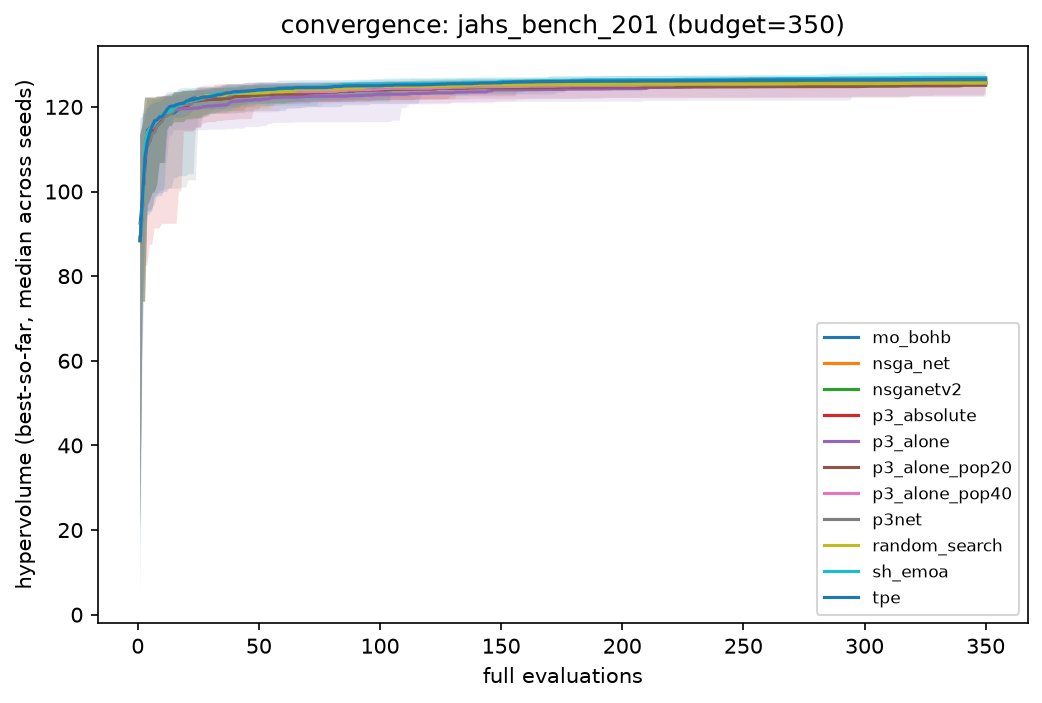
\includegraphics[width=\linewidth]{figures/convergence__jahs_bench_201__budget350.png}
    \caption{Median best-so-far relative hypervolume vs.\ full evaluations, all eleven arms, JAHS-Bench-201
    (CIFAR-10), budget~350. All arms reach a shared plateau within roughly the first tenth of the budget.}
    \label{fig:convergence-jahs-350}
\end{figure}

\subsection{Diagnosis}

\paragraph{The population pyramid spends the budget on random bootstrap.} Figure~\ref{fig:convergence-jahs-350}
shows every arm reaching a common plateau early, so the differences that matter are small and late. We therefore
measured what share of P3Net's proposals come from uniform-random level bootstrap rather than from
surrogate-guided mixing. Because level sizes grow geometrically, each new level is larger than all previous
levels combined, and filling it dominates the budget. The redesign described in
Section~\ref{sec:proposed-optimizer} -- warm-starting each new level from the current front and growing on a
hypervolume-contribution criterion rather than strict dominance -- was introduced in response to this, and all
reported numbers are from the grid re-run with it. Even so, the bootstrap share rises with budget on every search
space; on NAS-HPO-Bench-II it is 67.3\%, 77.6\%, 84.6\%, and 90.5\% at the four budgets, and at budget~350 it is
89.7\% (CIFAR-10), 91.7\% (Colorectal-Histology), 92.4\% (Fashion-MNIST), and 90.5\% (NAS-HPO-Bench-II). The
warm start does not change the growth rule itself, which is what forces the trend. This accounts directly for
the random-search-like behaviour above and for the pattern of losses widening with budget.

The evidence that this travels with the engine rather than with either surrogate is P3+abs.\ regressor. In an
earlier pass it ran on a flat, fixed-size population, and there it separated from random search in most cells.
Once rewritten to share P3Net's pyramid, it separates in none, and against P3Net itself it is indistinguishable
in all sixteen cells. With the engine confound removed, this grid shows no measurable advantage of the relative
surrogate over the absolute one. Conversely, the P3-alone arms use a fixed population and fail differently: they
stagnate on a small, repeatedly revisited set. Their median sweep count is 7--9 at budget~50 but 1508.5--2388.5
at budget~350, several times the budget itself, because most sweeps are served from the deduplication cache.
P3Net's wins over them are therefore at least partly broad random exploration beating a stalled narrow one, and
are not by themselves evidence for the relative surrogate.

\paragraph{The surrogate is additive and poorly calibrated.} The acceptance gate's precision -- the fraction of
surrogate-accepted modifications that turned out to improve -- is 0.498 over 14562 logged predictions:
indistinguishable from chance. It is highest while $|\mathcal{H}_t| \leq 30$ (0.551) and lower thereafter.
Magnitudes are worse than predicting the mean: $R^2$ between predicted and true $\delta$ is $-1.46$ (CIFAR-10),
$-2.08$ (Colorectal-Histology), $-3.28$ (Fashion-MNIST), and $-1.76$ (NAS-HPO-Bench-II). The error concentrates
at one pyramid level. At budget~350, predictions made while sweeping the level of size 16 have
$R^2=-4.71$ (MSE 766.7) against $R^2=+0.55$ (MSE 85.2) at size 2, roughly 9 times the error. That level is the
first whose sweep begins after a large, freshly bootstrapped population, when the linkage tree proposes subsets
for which few training pairs exist; this mechanism is plausible but not directly confirmed. Telescoping
accumulates error over the first steps of a chain (median squared error 26.5 at depth~1, 106.2 at depth~5) but
not monotonically beyond that.

Because $\hat\delta_F$ is linear in one-hot features, it cannot represent the joint effect of the coordinates
that linkage-guided crossover changes together, which is in tension with the premise of the crossover itself. As a
proxy for how much this matters per search space, we measure the out-of-sample $R^2$ gained by adding second-order
interaction terms touching at least one architecture edge to a main-effects model of $f_1$: $+0.016$ on
Fashion-MNIST, $+0.055$ on CIFAR-10, $+0.109$ on Colorectal-Histology, and $+0.259$ on NAS-HPO-Bench-II. This is
exactly the order in which P3Net's wins over its surrogate-free ablations weaken, from most complete on
Fashion-MNIST to none on NAS-HPO-Bench-II. The correspondence is observational; we did not intervene on it alone.
An arm that augments $\hat\delta_F$ with pairwise ``changed together'' interaction features, which fits a
constructed non-additive pattern that the plain model cannot represent, reaches significance against P3Net in 1
of 16 cells, in P3Net's favour. Added capacity did not translate into search performance.

\paragraph{Duplicate proposals are not what distinguishes P3Net.} Our initial hypothesis was that
dependency-aware variation would propose fewer duplicate genotypes. Mean proposal-time duplication is high for
the fixed-population P3 arms (P3-alone 0.734, P3-alone-pop20 0.448, P3-alone-pop40 0.187) and for SH-EMOA
(0.234), but P3Net (0.076) is not the lowest of the P3- and NSGA-II-engine arms: P3+abs.\ regressor (0.044),
NSGANetV2 (0.046), and NSGA-Net (0.038) all duplicate less. Whatever suppresses duplicates on the pyramid is not
specific to the relative surrogate.

\subsection{Isolation experiments}

The remaining candidate explanations are the joint genotype and the benchmark family. Both experiments below use
architecture-only NAS-Bench-201 through NATS-Bench~\citep{dong2021natsbench} ($n=6$ edge coordinates, no
$\Theta$), budgets 100 and 350, $R=30$, and the same statistical protocol; the best-known front is pooled within
this grid. Two deviations are forced by the benchmark interface: $f_2$ is FLOPs, as measured GPU
energy~\citep{bartnik2026evolutionary} is not a queryable field, and $f_1$ is test error. Because every arm is
scored identically, these deviations affect absolute values but not the comparison.

\begin{table}[t]
    \centering
    \footnotesize
    \caption{Architecture-only NAS-Bench-201. Relative hypervolume medians; Holm-corrected $p$ and Cliff's
    $\delta$ of the first arm against the second. No comparison rejects $H_0$.}
    \label{tab:isolation}
    \begin{tabular}{@{}llrrrr@{}}
        \toprule
        \textbf{Arm} & \textbf{vs.} & \textbf{Budget} & \textbf{Median} & \textbf{Adj.\ $p$} & \textbf{$\delta$} \\
        \midrule
        P3Net      & random search & 100 & 0.9851 & 0.9515 & $+0.016$ \\
        P3Net      & random search & 350 & 0.9923 & 0.7415 & $+0.118$ \\
        \midrule
        bartnik\_p3 & random search & 100 & 0.9856 & 1.0000 & $+0.113$ \\
        bartnik\_p3 & random search & 350 & 0.9935 & 0.5333 & $+0.273$ \\
        bartnik\_p3 & P3Net        & 100 & 0.9856 & 1.0000 & $+0.124$ \\
        bartnik\_p3 & P3Net        & 350 & 0.9935 & 0.9820 & $+0.222$ \\
        \bottomrule
    \end{tabular}
\end{table}

\paragraph{Removing the hyperparameter dimension.} Discretised hyperparameters enlarge $n$, and with it $\kappa$
and the space of linkage subsets, while plausibly carrying less combinatorial interaction than architecture edges.
If that diluted the linkage tree, removing $\Theta$ should help. It does not: P3Net still does not separate from
random search at either budget (Table~\ref{tab:isolation}), with both medians above 0.985.

\paragraph{The closest prior design.} Bartnik's SA-P3-GOMEA-class algorithm is documented to win on a search
space of this scale~\citep{bartnik2026evolutionary}. We reconstructed it as \texttt{bartnik\_p3}: canonical
single-individual-climbing P3, a random-forest absolute surrogate, and a quantile acceptance
gate~\citep{dushatskiy2021novelsurrogateassistedevolutionaryalgorithm}. This design avoids both of P3Net's
diagnosed defects: it has no geometrically bootstrapped levels, and its surrogate is not additive. On the
identical setup it does not separate from random search, nor from P3Net (Table~\ref{tab:isolation}). The null is
therefore not specific to P3Net's implementation; under this harness and baseline set, a design free of both
defects produces it as well.
